\documentclass[]{article}
\usepackage{lmodern}
\usepackage{amssymb,amsmath}
\usepackage{ifxetex,ifluatex}
\usepackage{fixltx2e} % provides \textsubscript
\ifnum 0\ifxetex 1\fi\ifluatex 1\fi=0 % if pdftex
  \usepackage[T1]{fontenc}
  \usepackage[utf8]{inputenc}
\else % if luatex or xelatex
  \ifxetex
    \usepackage{mathspec}
  \else
    \usepackage{fontspec}
  \fi
  \defaultfontfeatures{Ligatures=TeX,Scale=MatchLowercase}
\fi
% use upquote if available, for straight quotes in verbatim environments
\IfFileExists{upquote.sty}{\usepackage{upquote}}{}
% use microtype if available
\IfFileExists{microtype.sty}{%
\usepackage{microtype}
\UseMicrotypeSet[protrusion]{basicmath} % disable protrusion for tt fonts
}{}
\usepackage[margin=1in]{geometry}
\usepackage{hyperref}
\hypersetup{unicode=true,
            pdftitle={Ground breaking research!},
            pdfborder={0 0 0},
            breaklinks=true}
\urlstyle{same}  % don't use monospace font for urls
\usepackage{graphicx,grffile}
\makeatletter
\def\maxwidth{\ifdim\Gin@nat@width>\linewidth\linewidth\else\Gin@nat@width\fi}
\def\maxheight{\ifdim\Gin@nat@height>\textheight\textheight\else\Gin@nat@height\fi}
\makeatother
% Scale images if necessary, so that they will not overflow the page
% margins by default, and it is still possible to overwrite the defaults
% using explicit options in \includegraphics[width, height, ...]{}
\setkeys{Gin}{width=\maxwidth,height=\maxheight,keepaspectratio}
\IfFileExists{parskip.sty}{%
\usepackage{parskip}
}{% else
\setlength{\parindent}{0pt}
\setlength{\parskip}{6pt plus 2pt minus 1pt}
}
\setlength{\emergencystretch}{3em}  % prevent overfull lines
\providecommand{\tightlist}{%
  \setlength{\itemsep}{0pt}\setlength{\parskip}{0pt}}
\setcounter{secnumdepth}{0}
% Redefines (sub)paragraphs to behave more like sections
\ifx\paragraph\undefined\else
\let\oldparagraph\paragraph
\renewcommand{\paragraph}[1]{\oldparagraph{#1}\mbox{}}
\fi
\ifx\subparagraph\undefined\else
\let\oldsubparagraph\subparagraph
\renewcommand{\subparagraph}[1]{\oldsubparagraph{#1}\mbox{}}
\fi

%%% Use protect on footnotes to avoid problems with footnotes in titles
\let\rmarkdownfootnote\footnote%
\def\footnote{\protect\rmarkdownfootnote}

%%% Change title format to be more compact
\usepackage{titling}

% Create subtitle command for use in maketitle
\newcommand{\subtitle}[1]{
  \posttitle{
    \begin{center}\large#1\end{center}
    }
}

\setlength{\droptitle}{-2em}
  \title{Ground breaking research!}
  \pretitle{\vspace{\droptitle}\centering\huge}
  \posttitle{\par}
  \author{Kirien Whan\(^1\) and Famous Collaborators\(^2\)\\
1. KNMI\\
2. University}
  \preauthor{\centering\large\emph}
  \postauthor{\par}
  \predate{\centering\large\emph}
  \postdate{\par}
  \date{January 25, 2018}

\usepackage{rotating}

\usepackage{lscape}
\newcommand{\blandscape}{\begin{landscape}}
\newcommand{\elandscape}{\end{landscape}}

\usepackage{natbib}
\bibliographystyle{apalike}

\begin{document}
\maketitle
\begin{abstract}
The abstract text goes here\ldots{}.
\end{abstract}

\section{Introduction}\label{introduction}

Citing my own work (Whan et al. 2015). Can also use latex citations, but
then you need to run bibtex etc \citep{whan2015impact}.

\section{Data and Methods}\label{data-and-methods}

You can call R directly in-line like this, e.g.~We use 50 years of data.
Or you can call objects that have been defined in previous chunks like
this, e.g.~We use 50 years of data.

Including latex code directly is easy using dollar signs, e.g.~The Niño
3.4 index is the area averaged standardized SST anomalies from the
tropical Pacific (5\(^{\circ}\)N-5\(^{\circ}\)S,
170\(^{\circ}\)W-120\(^{\circ}\)W)

Referencing equations is easy as well since we can include latex code
directly. See equation 1:

\begin{enumerate}
\def\labelenumi{(\arabic{enumi})}
\tightlist
\item
  \[  ONETHING  = \max\limits_{j=1,..k}[OF.SOME.OTHER.THINGS] \]
\end{enumerate}

\section{Results}\label{results}

There are built in ways to do figure cross-referencing, but I found this
method best (using functions imported from the script
``functions\_markdownCrossRef.R'') (Figure 1). Referencing tables is
done like this (Table 1).

We find a relationship between ENSO and temperature (r = -0.4).

\section{Conclusions}\label{conclusions}

\section{References}\label{references}

\begin{figure}
\centering
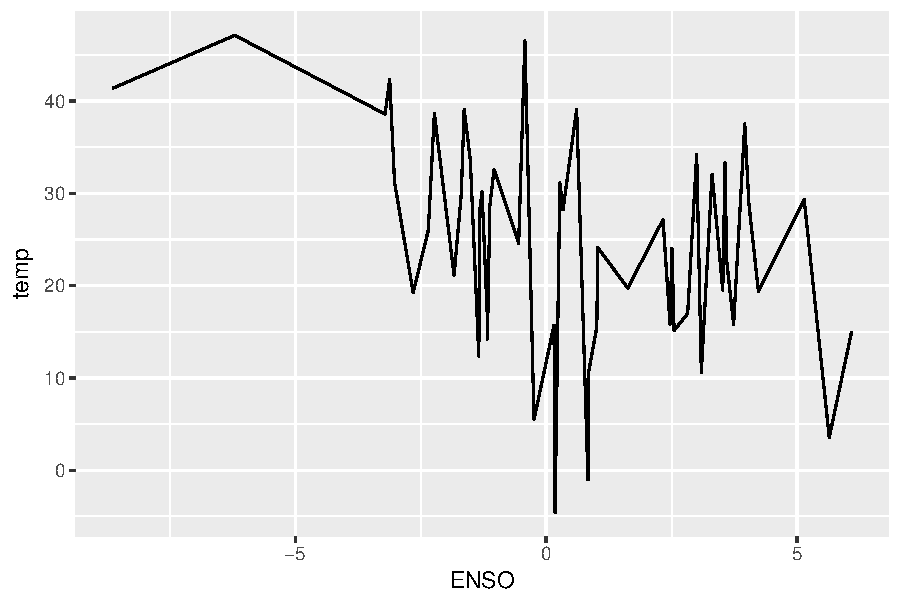
\includegraphics{example_files/figure-latex/makeplot-1.pdf}
\caption{The Correlation between ENSO and Temp}
\end{figure}

\hypertarget{refs}{}
\hypertarget{ref-whan2015impact}{}
Whan, Kirien, Jakob Zscheischler, Rene Orth, Mxolisi Shongwe, Mohammad
Rahimi, Ernest O Asare, and Sonia I Seneviratne. 2015. ``Impact of Soil
Moisture on Extreme Maximum Temperatures in Europe.'' \emph{Weather and
Climate Extremes} 9. Elsevier: 57--67.


\end{document}
